\chapter{Reconstruction} % 

The precise measurement of particles produced in the high energy collisions at the LHC 
is necessary to effectively execute the CMS physics programme. This requires high precision
reconstruction and identification of physics objects in a challenging environment containing
large numbers of different particles with a range of energies. The \alphat analysis 
relies directly on reconstruction of jets and \met for the signal region and on the 
reconstruction of leptons and photons to reject electroweak 
backgrounds and to define control regions.
This requires the use of information from all detector subsystems and state-of-the-art
techniques to allow the reconstruction, selection and calibration of these physics objects.


\section{Detector reconstruction}

The first stage in reconstructing the physics objects is to produce the necessary
input information from the detector subsystems. This takes the form of both the tracks, 
trajectories, of charged particles as well as the energy measurements from
calorimeter depositions. Specialist algorithms which suppress backgrounds, 
mitigate the effects of pileup and provide high resolution energy,
position and/or temporal measurements are used to optimise the precision of the 
measured quantities over a wide range of particle energies and momenta.

\subsection{Track reconstruction}

Charged particle tracks are reconstructed from the hits, considering the efficiency and resolution, 
using the iterative Combinatorial Track Finder (CTF) algorithm. The track reconstruction can be decomposed 
into four logical steps outlined below.

\begin{itemize}
\item Seeds are generated using either triplets of tracker hits or pairs of hits with an additional constraint 
from the beamspot or a pixel vertex. This gives an initial estimate of the trajectory with uncertainty \cite{tracker_early}.
\item Each seed is propagated outward through the tracker layers considering the current uncertainty in the trajectory.
In propagating, a uniform magnetic field as well as no energy loss or multiple Coulomb scattering effects are assumed.
The track parameters are updated with the best matching hit on each layer (if any) according to the Kalman filter formalism \cite{tracker_vertex}.
The search continues until either the boundary of the tracker is reached or no more compatible hits are found. If a minimum number
of valid hits are observed an inwards search is initiated for additional hits\cite{tracker_early}.
\item It is possible for a single charged particle track to be reconstructed more than once, starting either from different seeds or if
one seed develops into multiple track candidates. If the fraction of shared hits between two track candidates is greater
than 19\% (determined empirically) the track with fewer hits is discarded. If the number of hits is equivalent the track with
 the largest $\chi^2$ is discarded\cite{tracker_vertex}.
\item After the track candidates are built and cleaned the hits in each candidate are refitted using a Kalman filter and smoother. This 
avoids possible bias from the seeding stage \cite{tracker_vertex}.
\end{itemize}

The CTF performs six iterations to determine the tracks. Between each iteration any hits that are assigned to tracks in the
previous iteration are removed from the collection. The final track collection is then filtered to remove fake tracks using 
information on the number of hits, the $\chi^2$ and the compatibility of the track originating from a pixel vertex. The momentum 
resolution achieved is 0.7 (5)\% at 1 (1000) \GeV in the central region\cite{tracker_early}. Using a dataset of pions and muons from an early run 
at the LHC the tracking efficiency was measured as 98\% for tracks with $p_T > 500\MeV$ and $>99\%$ for tracks with $p_T > 2\GeV$\cite{tracker_eff}.

\subsection{Vertex Reconstruction}

As described in Sec.~\ref{lhc_intro}, the LHC produced an average of 25 simultaneous collisions per bunch crossing
during Run 2. It is essential to identify the Primary Vertex (PV) and the particles originating from it to allow 
particles from additional collisions to be rejected and to identify features such as displaced vertices. The tracks
are initially clustered using a deterministic annealing (DA) algorithm based on the points of closest approach of the 
tracks to the beamspot \cite{tracker_vertex}. The candidate vertices containing at least two tracks are then
fitted using an adaptive vertex fitter (AVF) to compute the best estimates of vertex parameters \cite{tracker_avf}. 
Each track in the vertex is assigned a weight between 0 and 1 corresponding to the likelihood that that track
belongs to the vertex. The tracks with weight near 1 are most consistent with the reconstructed vertex while
those that are least consistent have small weights. The number of degrees in the fit, defined as 

\begin{equation}
n_{dof} = -3 + 2 \sum_{i=1}^{\#tracks} wi,
\end{equation}

is an important parameter for distinguishing real proton-proton interactions from misclustered vertices as it is strongly corrected with
the number of tracks compatible with arising from the interaction region \cite{tracker_vertex}. The vertex
position and resolution determined using the AVF have been 
measured in early LHC data and compared with simulation as shown in Fig~\ref{fig:pvEffRes}.

\begin{figure}[hbt]
  \begin{center} 
   \subfigure[\label{fig:pvEff}]{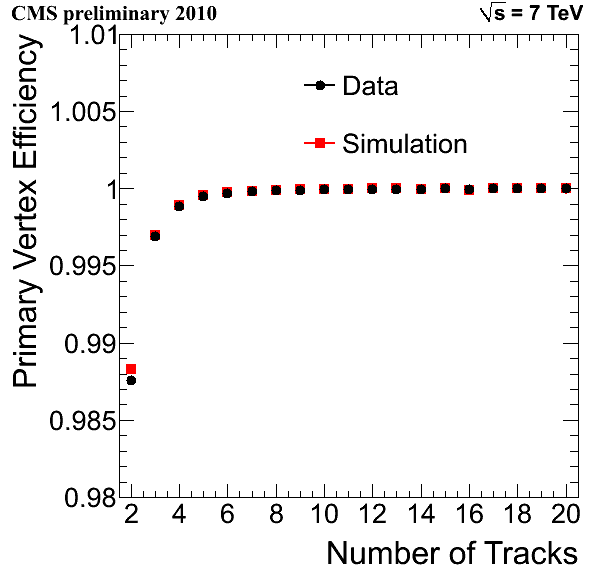
\includegraphics[width=0.5\textwidth]{Figures/detector/pvEff}}~
   \subfigure[\label{fig:pvRes}]{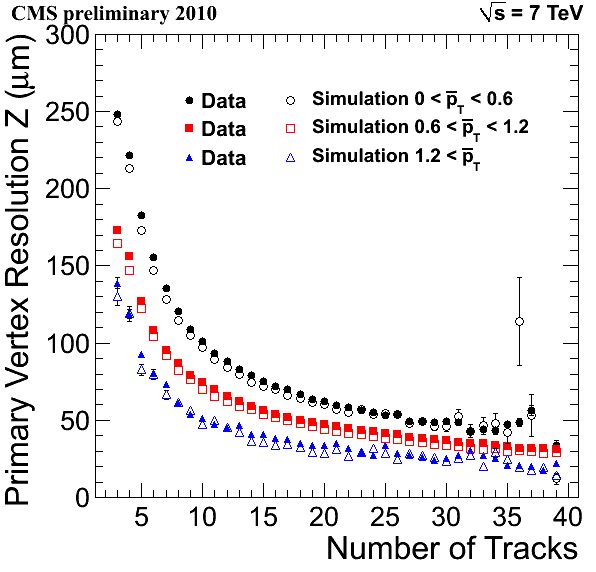
\includegraphics[width=0.5\textwidth]{Figures/detector/pvRes}}
   \caption{(a) Primary Vertex efficiency as a function of the number of associated tracks. (b) Primary Vertex 
   resolution in the z coordinate as a function of the number of associated tracks for three track $p_T$ scenarios \cite{tracker_seven}
   \label{fig:pvEffRes} }
  \end{center}
\end{figure}

The vertices are ordered according to the sum of the $p_T^2$ of the tracks associated to each vertex with the 
vertex with the highest $p_T^2$ taken as the primary vertex (PV). The position of the primary vertex can
be used for object identification and control of pile-up. Many CMS analyses, including the one in this 
thesis, make requirements that a good vertex is reconstructed from the tracks satisfying:

\begin{itemize}
\item A minimum number of degrees of freedom: $n_{dof} > 4$.
\item The collision to occur with $|z| < 24cm$ such that the primary vertex is near the interaction point in the longitudinal direction.
\item The collision to occur within a radial distance of $|d_{xy}| < 24cm$ from the beamline.
\end{itemize}

\subsection{Calorimeter reconstruction}

The calorimeters must reconstruct the energies of incident particles from the energy deposits made in the 
various subsystems. These deposits must be clustered and the measurement calibrated to provide 
details of the energy, position and timing of the incident particle. These can be used to complement 
the information from the tracker and provides necessary redundancy in the case of track
misreconstruction. For neutral particles the calorimeter subsystems provide the only measurement of
the particle properties.

The ECAL crystals are calibrated with both absolute and relative calibrations. Nine EB superclusters
and 500 EE crystals are calibrated using high energy electron beams to achieve a resolution of 0.5\% (1\%) for the EB (EE) components. 
The remainder undergo relative intercalibration to achieve a resolution of 1.4\%-1.8\% ($\sim5\%$) for the EB (EE) components. 
During running the response of the crystals changes due to radiation induced crystal-lattice defects which absorb the scintillation light. 
The crystal transparency is monitored to allow the impact on energy measurements to be assessed and corrected \cite{ecal_calib}. 
The HCAL components undergo a similar calibration to the ECAL crystals. Firstly a subset of the components are calibrated with
a 50 \GeV~pion beam and this is then extended to the remainder of the subsystem using a Co source \cite{hcal_beam}. Additional corrections
for the HCAL component are derived during LHC running \cite{hcal_calib}.

The reconstruction of the energy at the HCAL and ECAL relies on recording the amplified light pulses from the photodiodes over a 25ns time
sample. When operating with 25ns bunch spacing particle energies from previous or following bunch crossings can be integrated
into this sample, biasing the energy measurement. This effect is correcting by using a dedicated reconstruction that removes
the contributions from such Out Of Time Pileup (OOTPU)~\cite{hcal_timing,ecal_timing}. The 25ns sample is fitted including three pulse shape templates with
variable amplitude and arrival times with the central pulse corresponding to the triggered event. The timing distribution for
the ECAL hits above 1~\GeV, which is derived independently from the energy measurement, is shown in Figure~\ref{fig:timing_barrel_linear} showing that
contributions from OOTPU are rejected.

\begin{figure}
\centering
    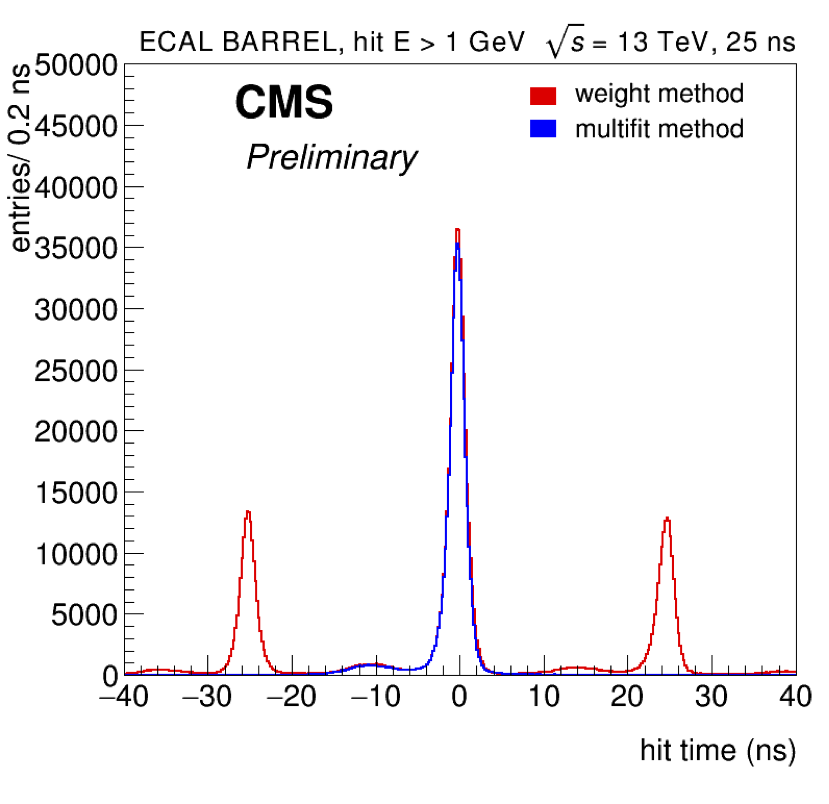
\includegraphics[width=0.8\textwidth]{./Figures/reconstruction/timing_barrel_linear.png}
  \caption{Timing distribution of the hits in the ECAL barrel with a reconstructed energy above 1\GeV~\cite{ecal_timing}.}
  \label{fig:timing_barrel_linear}
\end{figure}

\section{Physics object reconstruction}

The reconstructed tracks and calorimeters form the inputs to the reconstruction of the particles and 
jets that form the basis of the final selection of many analyses, including the analysis described 
in the thesis, referred to as physics objects. These are reconstructed using a combination of
dedicated local reconstruction algorithms as well as the global event Particle Flow algorithm, described in ??.
In addition, several WPs of selection criteria are defined for each physics object 
which provide a range of efficiencies and corresponding proportion of false positives. 

\subsection{Electron and photon reconstruction}

Photons and electrons interact similarly within the ECAL and so these objects follow similar reconstruction techniques.
Electrons are reconstructed by matching information in the tracker and ECAL
using two complementary techniques, an ECAL driven reconstruction described in this section (identical aside from tracking requirements
to the photon reconstruction) and a tracker-driven reconstruction performed with the PF algorithm described in section ??
which is optimal for low $p_T$ electrons. 

In the ECAL, both electron and photon candidates are formed by clustering energy deposits
from electromagnetic showers. Around 50\% of the photons convert into an electron-positron pair in the material proceeding the calorimeter
leaving an energy deposit that is widely spread in $\eta$ and $\phi$ \cite{electron_photon_reco}. 
For unconverted photons the deposits are fairly localised in $\eta$ and $\phi$. Electrons radiate
bremsstrahlung in the presence of the magnetic field and lose $33\%$ of their energy on average
in the central region and up to $86\%$ at $|\eta| = 1.4$. Their energy deposits are widely spread
in $\phi$ but narrow in $\eta$. The hybrid (multi) clustering algorithm exploits this characteristic to
reconstruct high energy electrons and photons in the barrel (endcap). The hybrid algorithm
uses a seed crystal and clusters up to ten strips (dominoes) of $1\times3$ or $1\times5$ ($\phi\times\eta$) within 
$\Delta\phi < 0.3$ from the seed. Any domino with an energy under $100\MeV$ ~is discarded. The dominoes
are themselves clustered in $\phi$ provided each disconnected subcluster has a seed domino of energy $>350\MeV$.
The combination of these subclusters is referred to as a supercluster. The multi reconstruction in the endcap 
follows a similar procedure using $5\times5$ grids of crystals. 

Superclusters which can be associated to tracks originating from the primary vertex are reconstructed as electrons.
As electrons lose energy through the non-Gaussian bremsstrahlung process the Kalman filter is innapropriate and
so the specialist track reconstruction Gaussian Sum Filter algorithm is used. This allows the total energy of
electrons to be reconstructed including the component lost through bremsstrahlung. The photons are identified 
through inverting the track matching criteria of the supercluster. In the endcaps, additional information
is used from the preshower when reconstructing the energy.

Additional selections are applied on all reconstructed electrons and photons to suppress backgrounds.
For electrons these are mainly composed of misreconstructed jets, secondary electrons from photon
conversions and semi-leptonic decays of heavy quarks. As electrons are mainly contained within 
the ECAL a requirement on the ratio of energies in the ECAL and HCAL provides a strong veto of hadronic
backgrounds. In addition, requirements are made on the matching track such that the transverse distance from 
the primary vertex is $d_{xy} < 0.0261$ ($d_{xy} < 0.118$) and the longitudinal distance is $d_z < 0.041$
($d_z < 0.822$) for the barrel (endcap). These impact parameter requirements ensure the track originates from 
the primary vertex. Several variables that rely on the shower shape and cluster
width are used to reject fakes including the $\sigma_{i\eta i\eta}$ which is the second moment of the log-weighted
distribution of crystal energies calculated in the $5\times5$ matrix around the most energetic crystal. The value of
 $\sigma_{i\eta i\eta}$ is larger on average for neutral meson decay to two collimated photons.

\subsection{Muon reconstruction}
\label{muon_reco}
Muons are MIPs, leaving minimal energy deposits in the calorimetry subsystems, and travelling through
the entire detector. The muons are therefore reconstructed using a combination of the inner tracker
and muon systems. Two algorithms are used to give complementary efficiency across the momentum spectrum,
the 'the outside-in' Global Muon algorithm and 'the inside-out' Tracker 
Muon algorithm \cite{muon_reco}.

The outside-in algorithm begins with identifying a tracker match for each muon track. Hits in muon
chambers are used to define standalone-muon tracks. These are then matched with tracker tracks
by comparing parameters of the two tracks propagated onto a common surface. The hits from
both systems are then combined and a global muon fit is performed using a Kalman filter. The momentum 
resolution is significantly improved by the global fit over a tracker only fit for muons of $p_T < 200\GeV$
 \cite{CMS,muon_reco_cosmic}. 

The inside-out algorithm selects all tracks satisfying $p_T > 0.5\GeV$ and $p > 2.5\GeV$. These are then 
extrapolated to the muon system taking into account effects from the magnetic field, multiple Coulomb scatting
in the detector material and the average expected energy loses. If at least one muon segment matches 
the extrapolated track the track qualifies as a Tracker Muon. Tracker Muon reconstruction is more efficient
than global muon reconstruction for low momenta of $\sim p< 5\GeV$. This is due to only requiring one segment
of the muon system while global muon reconstruction is more efficient for higher energy muons which are likely
to pass through several muon stations \cite{muon_reco}.

In order to ensure the muons are prompt (produced in by the hard process such as vector boson decay) rather
than non-prompt (produced from the in-flight decays of hadrons, taus or heavy quarks) and to reject fakes
caused by the punch through of hadronic particles, additional selections are made. These include quality
selection on the $\chi^2$ of the muon track, a minimum number of valid hits as well as requirements
on the impact parameters $d_{xy} < 0.05 cm$ and $d_{z} < 0.1 cm$ aimed at ensuring prompt muons.

Muons must be reconstructed through either the Global or Tracker Muon algorithm. In combination, and
including additional selections, these provide an of $>95\%$ for
reconstructing a muon with $p_T$ larger than a few \GeV~over the full $\eta$ range covered by the
muon system and a fake rate from hadrons of $<1\%$ \cite{muon_reco}.

\section{Particle Flow}

The particle flow algorithm combines the inputs from dedicated track reconstruction and calorimeter clustering
algorithms using all detector subsystems to identify and reconstruct all stable particles in the event.
Despite hundreds of different particle species being produced by collisions at the LHC only a small fraction
have sufficient lifetimes and interactions with the detector to be directly measured. The predominant species
measured by the CMS detector are: $\gamma$, $e^{\pm}$, $\mu^{\pm}$, $\pi^{\pm}$, $K^{\pm}$, $p^{\pm}$, $K^{0}$
and $n$, classified by the PF algorithm into five categories of photons, electrons, muons, charged hadrons and neutral hadrons. 
The identification and measurement of the properties of these particles is optimised by taking advantage of the complementarity of 
different subsystems in various kinematic regimes and geometries over the performance achievable with 
any one subsystem alone. The output list of the individual particles is similar to that provided
when generating Monte Carlo events. This can then be used to as an input for further reconstruction processes
such as building jets, determining  \met~, determining jets originating from bottom quarks (b tag) and quantifying
charged lepton isolation. The algorithm is described fully in \cite{pf_proc,pf_pas}.

Effective track reconstruction forms the core of the particle-flow algorithm. The CMS detector, with a strong magnetic field
and large silicon tracker, is highly capable of the efficient track reconstruction required. In addition, the high 
granularity ECAL allows effective separation of photons from charged particles, even inside jets of several hundred
\GeV, and the entire calorimetry system is included within the solenoid, allowing an uninterrupted measurement 
of the particle energy flow.

The PF algorithm utilises a specific clustering algorithm for calorimeter deposits which is performed separately 
in each calorimeter sub-detector. First, cluster seeds are identified as local cell maxima over a threshold energy.
Second, these are grown into topological clusters by aggregating any cells with at least one side in common with
a cell already in the cluster and with energy above a given sub-detector dependant threshold. Finally, the 
total energy in each topological cluster is shared between all encompassed seed clusters according to the 
cell-cluster distance to form a PF cluster for each seed. These PF clusters form the inputs along with 
reconstructed tracks for PF candidates.

The PF reconstruction uses a link algorithm to iteratively check compatibility of charged particle tracks, and/or
calorimetry clusters and/or muon tracks. These elements must be connected while avoiding any double counting. 
The link algorithm is performed on every pair of elements in the event and defines a distance between them
that quantities the quality of the link. This is used to produce blocks of elements linked directly 
or indirectly. The blocks are constructed depending on the subsystems being linked as described below:

\begin{itemize}
\item A link between a charged particle track and calorimeter deposit is made by extrapolating the last measured
hit in the tracker through the calorimetry systems. The track is linked to a cluster if the calorimeter position
is within the cluster boundaries. The link distance is defined as the distance in the ($\eta,\phi$) plane between
the extrapolated track position and cluster position.
\item Clusters caused by bremsstrahlung photons emitted by electrons are associated to the track by extrapolating
the tangents to the track from the intersection points of the track and tracker layers to the ECAL. The distance measure
is the same as defined above.
\item Calorimeter clusters are linked between HCAL and ECAL or between ECAL and PS clusters by establishing whether
the cluster in the more granular calorimeter is within that of the less granular. The link distance is defined
as the distance in the ($\eta,\phi$) plane between the cluster positions
\item Charged particles tracks are associated with muon tracks following the Global Muon algorithm defined in 
Section~\ref{muon_reco}. In this case the $\chi^2$ of thew global fit defines the link distance.
\end{itemize}

With the blocks defined, the algorithm for reconstruction and identification of the set of particles from each
block, which form a global description of the event, proceeds as follows:

\begin{itemize}
\item First, each global muon is defined as a PF muon if its combined momentum is compatible with the momentum 
from the tracker only within three standard deviations. The track is removed from the block and expected energy depositions
along the path of the muon in the calorimeters are subtracted (measured with cosmic ray muons to be 3 GeV and 0.5 GeV respectively for the 
ECAL and HCAL).
\item Electrons are then identified. Tracks are pre-identified as electron tracks based on their 
characteristics within the tracker. Such tracks are refitted with a Gaussian-Sum Filter and extrapolated to the ECAL. 
Several tracking and calorimetric variables are then used to perform a final identification of PF electrons. The track
and ECAL clusters (including those from bremsstrahlung) are removed from the block.
\item The remaining tracks undergo additional quality criteria and are connected to ECAL and HCAL clusters. 
If calorimetric deposits are linked with a track a PF charged hadron is identified. 
\item The detection of neutral particles in addition to the PF charged hadron 
relies on a comparison of the momentum of the tracks and the calibrated energy in the calorimeters. 
If the momentum of the track is compatible with the calorimeter deposits within measurement uncertainties 
a PF charged hadron is identified. The momentum and energy are then taken from the track momentum under a 
charged pion hypothesis. If the calibrated calorimetric energy is significantly in excess of this energy, considering
the calorimetric resolution, a PF photon and possibly a neutral hadron are also identified. 
If the energy excess is larger than the total ECAL energy, a PF photon is created with the ECAL energy and a 
PF neutral hadron is created taking the remainder of the excess. Otherwise, only a PF photon is created with the energy of the excess.
\item Any remaining ECAL and HCAL clusters give rise to PF photons and PF neutral hadrons respectively.
\end{itemize}

\subsection{Pileup estimation}

In reconstructing the hard process it is important to remove contributions from additional
vertices. The input from the particle flow reconstruction can be used to identify 
charged hadrons which do not originate from the primary vertex. However, the vertex 
for neutral particles cannot be determined. Instead, the ratio of neutral and 
charged particles can be measured in simulation and a correction factor determined.
This is necessary as neutral particles compose $\sim 50\%$ of the pileup in the barrel.
An additional form of pileup subtraction relies on an estimate of the local energy density 
of pileup, $\rho$, which can then be used to correct physics objects covering an area,
A, as

\begin{equation}
p_T^{Corr} = p_T^{Raw} - \rho \cdot A,
\end{equation}

where the values for $\rho$ are determined in Rub 2 by partitioning the detector into a square grid of spacing
0.55 and calculating the median energy of the energy density of all PF-candidates within each cell \cite{fastjet}.

\subsection{Isolation}

The level of hadronic activity around a lepton provides an effective method to distinguish between prompt and non-prompt leptons.
This level of activity is measured by the isolation of the lepton which is defined by the fraction of energy
in a cone around the lepton to the energy carried by the lepton itself.

The standard method of measuring isolation used during Run 2 by CMS is the PF isolation, $I_{PF}^{rel}$,
defined within a cone of radius $\Delta R$ as 

\begin{equation}
I_{PF}^{rel} = \frac{1}{p_T^{l}}\left[ \sum_{PF_{PV}}p_T^{CH} +  \sum_{PF}p_T^{NH} +  \sum_{PF}p_T^{\gamma} -  \sum_{PU}p_T^{\text{Neutral}}\right]
\end{equation}

where $p_T^{l}$,$p_T^{CH}$,$p_T^{NH}$,$p_T^{\gamma}$ are the momentum of the lepton, charged hadrons, neutral hadrons and photon respectively.
A subtraction of the neutral pileup must be made as neutral particles cannot be associated with the PV. The $\Delta \beta$ correction
and Effective Area correction are two methods used by CMS to estimate and correct for the neutral pileup contribution. The delta $\Delta \beta$
correction estimates the energy from the neutral hadrons from the charged hadron component, based on simulation, as

\begin{equation}
\sum_{PU}p_T^{\text{Neutral}} = \frac{1}{2} \sum_{PF_{PU}}p_T^{CH}
\end{equation}

while the effective area corrects the expected neutral pileup energy based on the footprint of the particle, $A_{eff}$ and the grid pileup
energy density computed from neutral particles, $\rho_{grid}^{\text{Neutral}}$

\begin{equation}
\sum_{PU}p_T^{\text{Neutral}} = \rho_{grid}^{\text{Neutral}}\cdot A_{eff}.
\end{equation}

the cone size may be fixed (relative isolation) or dependant on the \pt~of the particle (mini-isolation). The use of mini-isolation
accounts for the increasing collinearity of the hadronic decays of boosted particles. 

\subsection{Isolated tracks}

Unreconstructed (lost) leptons form a large background for hadronic searches. Lost leptons can be caused by both acceptance 
effects and by misreconstruction of processes including $e^{-}$, $\mu^{-}$ decays and hadronic decays of $\tau$ leptons. 
Typically, even if not associated to the lepton its track will still be reconstructed. Additionally, prompt leptons 
tend to be isolated and so the lost lepton background from misreconstructed leptons can be mitigated by the veto of high
energy isolated charged tracks. Isolated tracks are defined from PF candidates associated with the PV and 
which pass track quality selection but are not identified as leptons.

\section{Jet reconstruction} 

As the LHC is a hadron collider, most events will involve the production of quarks and gluons. As discussed in
Section ?? these strongly interacting particles hadronise into collimated jets of particles. As described 
in the following section, the properties  of the original parton which formed the jet can be reconstructed through the combination
of all of the particles that form the jet. In order for the properties of the jet to be theoretically tractable the
reconstruction algorithm has to satisfy the requirements of infrared safety, insensitive to the addition of 
soft particles, and collinear safety, insensitive to collinear splitting of particles.

\subsection{Jet clustering}

To acheive infrared collinear safety, CMS uses a sequential recombination algorithm \cite{antikt}. The input clusters can represent
the momenta of particles, calorimeter energy deposits or previously clustered 4-vectors. Interjet distances,

\begin{equation}
d_{ij} = min\left[p^r_{T_i},p^r_{T_j}\right]\left(\frac{\Delta R_{ij}}{R}\right)^2,
\end{equation}

between each pair of clusters i and j are defined, as well as beam-jet distances, 

\begin{equation}
d_{iB} = p^r_{T_i}
\end{equation}
where the $r$ parameter depends on the specific algorithm used, R determines the maximum distance
for clustering pairs and $p_{T_i}$ is the transverse momentum of the cluster. The algorithm then proceeds
as follows:
\begin{itemize}
\item Calculate and rank all the distances, $d_{ij}$ and $d_{iB}$ for all clusters in the event
\item If the smallest distance is an interjet distance combine clusters i and j into a new cluster and recalculate distances
\item If the smallest distance is a beam-jet cluster i is considered to be a final state jet and is removed from the event. Distances 
are then recalculated.
\end{itemize}

These steps are repeated until no clusters remain. The algorithm used for the analysis in this thesis (and for most CMS analyses) is 
the $anti-k_T$ algorithm for which $r=2$. The size of the jets is $R=0.4$ which is determined through optimising capture of all particles
associated with the jet and resilience against pileup. CMS uses jets with inputs from PF candidates (PF jets) and calorimeter deposits (Calo jets).
As shown in figure ** PF jets perform significantly better than calo jets. This is due to the significant position and energy resolution 
improvements possible with the tracker. PF jets are therefore used in offline analysis while calo jets are used only in HLT reconstruction
where latency restrictions forbid the construction of the PF candidates. 

To reject jets which are badly reconstructed or originate from detector noise additional selections are made on the jet. These include at least
two PF candidates, the fraction of energy from neutral hadrons and photons < 99\%,  charged hadron fraction > 0 and charged particle multiplicity > 0.
The rate of fake jets is reduced by 84\% while maintaining $> 99\%$ efficiency for jets from quarks and gluons.

\subsection{Jet energy corrections}

The energy of the clustered jets will not conform to the true partonic energy but instead is approximately Gaussian distributed around this value.
This is due to variation in response in different sections of the detector, at worst, losses in uninstrumented sections of the detector, as well as 
random fluctuations in the particle composition during hadronisation. To recover the true value Jet Energy Corrections (JECs) are applied using the functional
form \cite{jec}

\begin{equation}
\label{equ:jec}
  p_{\mu}^{\rm{cor}}=C_{\rm{offset}}\left(\pt^{\rm{raw}}\right)\cdot C_{\rm{rel}}\left(\eta\right)\cdot C_{\rm{abs}}\left(\pt'\right)\cdot C_{\rm{res}}\left(\pt'',\eta\right)\cdot p_{\mu}^{\rm{raw}}.
\end{equation}

where each $C$ in the equation represents a correction corresponding to offset, relative, absolute and residual for $C_{offset}$, $C_{rel}$, $C_{abs}$ and $C_{res}$ respectively, 
 ($p_{\mu}^{raw}$) $p_{\mu}^{corr}$ is the (un)corrected jet 4-momentum, $p'_T$ is the $p_T$ after the offset and relative corrections and  $p'_T$ is the $p''_T$ after
all corrections except the residual. These are described in more detail below \cite{jec2}:

\begin{itemize}
\item The $C_{offset}$ is the first step in the chain. Its purpose is to remove energy contributions not associated with the hard scattering from sources
such as noise and pileup. The pileup contributions are removed using Charged Hadron Subtraction (CHS) where PF candidates not associated to the PV
are removed before clustering and the jet area method. The jet area method removes neutral component of pileup from the jets by subtracting $\rho \cdot A_j$
from the $p^{raw}_T$, where $A_j$ is the active area of the jet and $\rho$ is the average pileup energy density, determined from the median energy of PF candidates
across the detector. 
\item The $C_{rel}$ is used to make the energy response uniform in $\eta$ for all jets using MC truth corrections derived from QCD dijet events.
\item The $C_{abs}$ is used to correct the energy response as a function of jet $p_T$. This is done using \zj~and \gj~events as for
these processes the boson $p_T$ is well known which can be used to balance the $p_T$ of the reconstructed jet.
\item The $C_{res}$ is used to correct residual differences between the responses in both $p_T$ and $\eta$ for data and MC and applied in data only.
\end{itemize}

Each correction has associated systematic and statistical uncertainties. These are added in quadrature to define the overall jet energy uncertainty. The 
overall uncertainty is shown in Fig~\ref{fig:jec_unc}.

\begin{figure}
\centering
    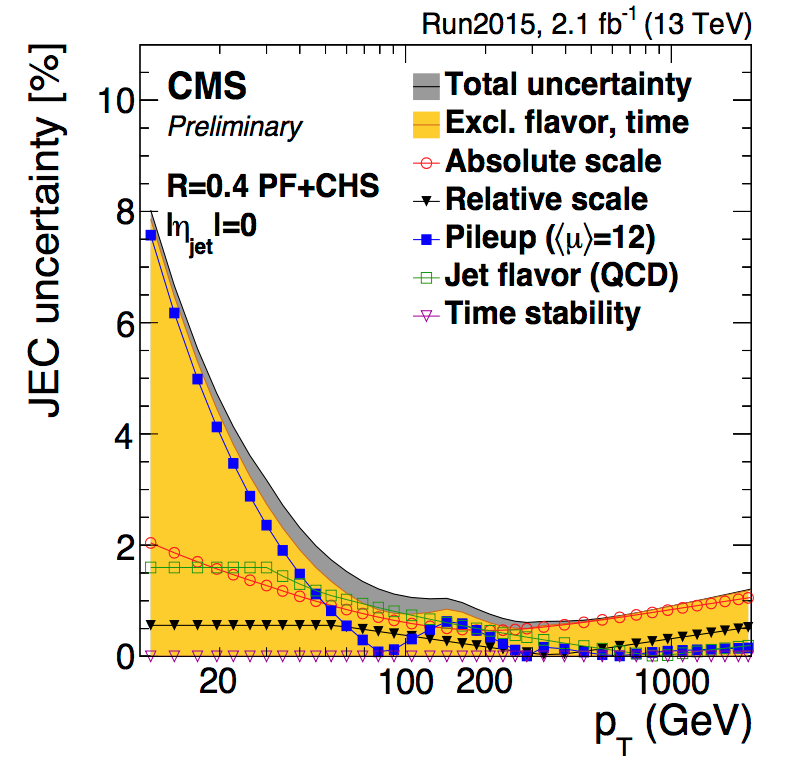
\includegraphics[width=0.8\textwidth]{./Figures/reconstruction/jec_unc.png}
  \caption{\label{fig:jec_unc} The overall uncertainty in the corrections applied to MC from Equation~\ref{equ:jec} shown in the orange solid curve. The pileup uncertainty dominates
for $p_T < 50\GeV$ while for higher values of $p_T$ the absolute and relative scale dominate \cite{jec_fig}.}
\end{figure}
